% Options for packages loaded elsewhere
\PassOptionsToPackage{unicode}{hyperref}
\PassOptionsToPackage{hyphens}{url}
\PassOptionsToPackage{dvipsnames,svgnames,x11names}{xcolor}
%
\documentclass[
  10,
  a4paper,
]{article}

\usepackage{amsmath,amssymb}
\usepackage{lmodern}
\usepackage{iftex}
\ifPDFTeX
  \usepackage[T1]{fontenc}
  \usepackage[utf8]{inputenc}
  \usepackage{textcomp} % provide euro and other symbols
\else % if luatex or xetex
  \usepackage{unicode-math}
  \defaultfontfeatures{Scale=MatchLowercase}
  \defaultfontfeatures[\rmfamily]{Ligatures=TeX,Scale=1}
\fi
% Use upquote if available, for straight quotes in verbatim environments
\IfFileExists{upquote.sty}{\usepackage{upquote}}{}
\IfFileExists{microtype.sty}{% use microtype if available
  \usepackage[]{microtype}
  \UseMicrotypeSet[protrusion]{basicmath} % disable protrusion for tt fonts
}{}
\makeatletter
\@ifundefined{KOMAClassName}{% if non-KOMA class
  \IfFileExists{parskip.sty}{%
    \usepackage{parskip}
  }{% else
    \setlength{\parindent}{0pt}
    \setlength{\parskip}{6pt plus 2pt minus 1pt}}
}{% if KOMA class
  \KOMAoptions{parskip=half}}
\makeatother
\usepackage{xcolor}
\usepackage[lmargin=2cm,rmargin=2cm]{geometry}
\setlength{\emergencystretch}{3em} % prevent overfull lines
\setcounter{secnumdepth}{-\maxdimen} % remove section numbering
% Make \paragraph and \subparagraph free-standing
\ifx\paragraph\undefined\else
  \let\oldparagraph\paragraph
  \renewcommand{\paragraph}[1]{\oldparagraph{#1}\mbox{}}
\fi
\ifx\subparagraph\undefined\else
  \let\oldsubparagraph\subparagraph
  \renewcommand{\subparagraph}[1]{\oldsubparagraph{#1}\mbox{}}
\fi


\providecommand{\tightlist}{%
  \setlength{\itemsep}{0pt}\setlength{\parskip}{0pt}}\usepackage{longtable,booktabs,array}
\usepackage{calc} % for calculating minipage widths
% Correct order of tables after \paragraph or \subparagraph
\usepackage{etoolbox}
\makeatletter
\patchcmd\longtable{\par}{\if@noskipsec\mbox{}\fi\par}{}{}
\makeatother
% Allow footnotes in longtable head/foot
\IfFileExists{footnotehyper.sty}{\usepackage{footnotehyper}}{\usepackage{footnote}}
\makesavenoteenv{longtable}
\usepackage{graphicx}
\makeatletter
\def\maxwidth{\ifdim\Gin@nat@width>\linewidth\linewidth\else\Gin@nat@width\fi}
\def\maxheight{\ifdim\Gin@nat@height>\textheight\textheight\else\Gin@nat@height\fi}
\makeatother
% Scale images if necessary, so that they will not overflow the page
% margins by default, and it is still possible to overwrite the defaults
% using explicit options in \includegraphics[width, height, ...]{}
\setkeys{Gin}{width=\maxwidth,height=\maxheight,keepaspectratio}
% Set default figure placement to htbp
\makeatletter
\def\fps@figure{htbp}
\makeatother
\newlength{\cslhangindent}
\setlength{\cslhangindent}{1.5em}
\newlength{\csllabelwidth}
\setlength{\csllabelwidth}{3em}
\newlength{\cslentryspacingunit} % times entry-spacing
\setlength{\cslentryspacingunit}{\parskip}
\newenvironment{CSLReferences}[2] % #1 hanging-ident, #2 entry spacing
 {% don't indent paragraphs
  \setlength{\parindent}{0pt}
  % turn on hanging indent if param 1 is 1
  \ifodd #1
  \let\oldpar\par
  \def\par{\hangindent=\cslhangindent\oldpar}
  \fi
  % set entry spacing
  \setlength{\parskip}{#2\cslentryspacingunit}
 }%
 {}
\usepackage{calc}
\newcommand{\CSLBlock}[1]{#1\hfill\break}
\newcommand{\CSLLeftMargin}[1]{\parbox[t]{\csllabelwidth}{#1}}
\newcommand{\CSLRightInline}[1]{\parbox[t]{\linewidth - \csllabelwidth}{#1}\break}
\newcommand{\CSLIndent}[1]{\hspace{\cslhangindent}#1}

\usepackage{booktabs}
\usepackage{longtable}
\usepackage{array}
\usepackage{multirow}
\usepackage{wrapfig}
\usepackage{float}
\usepackage{colortbl}
\usepackage{pdflscape}
\usepackage{tabu}
\usepackage{threeparttable}
\usepackage{threeparttablex}
\usepackage[normalem]{ulem}
\usepackage{makecell}
\usepackage{xcolor}
\usepackage{caption}
\usepackage{graphicx}
\usepackage{siunitx}
\usepackage{hhline}
\usepackage{calc}
\usepackage{tabularx}
\usepackage{adjustbox}
\usepackage{hyperref}
\makeatletter
\makeatother
\makeatletter
\makeatother
\makeatletter
\@ifpackageloaded{caption}{}{\usepackage{caption}}
\AtBeginDocument{%
\ifdefined\contentsname
  \renewcommand*\contentsname{Table of contents}
\else
  \newcommand\contentsname{Table of contents}
\fi
\ifdefined\listfigurename
  \renewcommand*\listfigurename{List of Figures}
\else
  \newcommand\listfigurename{List of Figures}
\fi
\ifdefined\listtablename
  \renewcommand*\listtablename{List of Tables}
\else
  \newcommand\listtablename{List of Tables}
\fi
\ifdefined\figurename
  \renewcommand*\figurename{Figure}
\else
  \newcommand\figurename{Figure}
\fi
\ifdefined\tablename
  \renewcommand*\tablename{Table}
\else
  \newcommand\tablename{Table}
\fi
}
\@ifpackageloaded{float}{}{\usepackage{float}}
\floatstyle{ruled}
\@ifundefined{c@chapter}{\newfloat{codelisting}{h}{lop}}{\newfloat{codelisting}{h}{lop}[chapter]}
\floatname{codelisting}{Listing}
\newcommand*\listoflistings{\listof{codelisting}{List of Listings}}
\makeatother
\makeatletter
\@ifpackageloaded{caption}{}{\usepackage{caption}}
\@ifpackageloaded{subcaption}{}{\usepackage{subcaption}}
\makeatother
\makeatletter
\@ifpackageloaded{tcolorbox}{}{\usepackage[many]{tcolorbox}}
\makeatother
\makeatletter
\@ifundefined{shadecolor}{\definecolor{shadecolor}{rgb}{.97, .97, .97}}
\makeatother
\makeatletter
\makeatother
\ifLuaTeX
  \usepackage{selnolig}  % disable illegal ligatures
\fi
\IfFileExists{bookmark.sty}{\usepackage{bookmark}}{\usepackage{hyperref}}
\IfFileExists{xurl.sty}{\usepackage{xurl}}{} % add URL line breaks if available
\urlstyle{same} % disable monospaced font for URLs
\hypersetup{
  pdftitle={Regional and Urban Economics},
  pdfauthor={Sindre Halvorsen Øveraas , Sebastian Mena Fløysand, Alen Colakovic \& Mona Lisa Jones},
  colorlinks=true,
  linkcolor={blue},
  filecolor={Maroon},
  citecolor={Blue},
  urlcolor={Blue},
  pdfcreator={LaTeX via pandoc}}

\title{Regional and Urban Economics}
\usepackage{etoolbox}
\makeatletter
\providecommand{\subtitle}[1]{% add subtitle to \maketitle
  \apptocmd{\@title}{\par {\large #1 \par}}{}{}
}
\makeatother
\subtitle{Dental industry}
\author{Sindre Halvorsen Øveraas , Sebastian Mena Fløysand, Alen
Colakovic \& Mona Lisa Jones}
\date{}

\begin{document}
\maketitle
\ifdefined\Shaded\renewenvironment{Shaded}{\begin{tcolorbox}[sharp corners, frame hidden, breakable, boxrule=0pt, borderline west={3pt}{0pt}{shadecolor}, enhanced, interior hidden]}{\end{tcolorbox}}\fi

\begin{verbatim}
Warning: One or more parsing issues, see `problems()` for details
\end{verbatim}

\hypertarget{abstract}{%
\subsection{Abstract}\label{abstract}}

There are several factors to take in to consideration when deciding
where a dental practice should be located. Spatial competition is a
critical consideration in regional economics. Some of the factors
influencing the decision making is retail agglomeration attributes,
spatial monopoly and the attractiveness of a particular place of
interest. This study aims to examine the dental industry and find the
strategy most profitable for the dental industry.

The study utilize a quantitative research approach, employing spacial
explanatory data analysis techniques to determine the location decisions
of firms. Geographical data was collected from locations in Norway
showing all dentists, central places, retail agglomeration and other
points of interest such as the government regulated wine monopoly.
Combined with regional income data a spatial regression analyses was
used to identify the factors influencing the location decisions of
firms.

Furthermore, the result indicates the distance to retail agglomeration
areas and central places playes a significant role in the location
decisions for firms. Firms are more likely to locate closer to these
areas, which offer access to a larger customer base and lower cost of
transportation. However, the results also suggest other factors, such as
market size and completion also influence the location decisions for
firms.

The studies findings have particular implications for policy-makers,
developer, and dental practises seeking to maximize profits through
strategic decisions. By understanding the importance of proximity to
retail agglomeration areas and central places, these stakeholders can
make informed decisions that benefit the local economy and improve
competitiveness of the region. Perhaps more importantly prevent
agrassive retail agglomeration areas from ``killing down town''.

\hypertarget{introduction}{%
\subsection{Introduction}\label{introduction}}

Our main task in this assignment is to perform an analysis of geospatial
determinants of firm activity. More specifically we are to focus on the
Norwegian dental industry in this regard, and see how geospatial
determinants such as distances to shopping malls and CBDs (Central
Business Districts), as well as population density can determine dental
businesses income and general financial operations. As an example,
central questions in this assignment will be; ``Is it more beneficial to
be highly centralized in urban areas with high population density and
many competitors, or is it a greater advantage to be less centralized to
the advantage that the nearest competing company is considerably further
away?'', ``Which determinants appear to be most significant for economic
benefit?''

The theoretical framework for this study draws on Marshall's
agglomeration principles, which emphasize spatial aspects of economic
growth. Hotelling's game theory is used to explain spatial competition
by location. Furthermore, adding the hybrid model whereas firms compete
both in location and price, with consumers having a transportation cost
and firms producing differentiated products. Alsonso's bid-rent model
and gravitational models also provides insights into how dentists or
other retailer makes location decisions in the context of regional
growth.

The dental industry provides an interesting industry to study for this
research because of its unique characteristics. Dental practices require
a high degree of specialization and expertise. At the same time, they
need to be easily accessible to consumers. Shopping malls and central
places offer a continent location for dental practices that said
competition for prime locations can be intense and push some in to
spatial monopoly.

The result of this study indicates that dentist's with the highest
income are usually located in central places in big cities. The findings
are in line with already exciting theories especially supporting the
gravitational models and agglomeration attributes. ?????? Proving a
central location within large cities are the best location to maximize
profit for Dental practices. ???

\textbf{Hypothesis}

The location choice of firms providing service to end consumers,
significantly determine their ultimate growth potential.

\textbf{Research question}

What is the most profitable location for dental practice?

\hypertarget{theoretical-framework}{%
\subsection{Theoretical Framework}\label{theoretical-framework}}

Location theory gives regional economics its scientific disciplinary
identity and constitutes its theoretical methodological core Capello
(2011). It has typically microeconomic foundation and uses theoretical
models as well as adopting a statistical and geographical approach
Capello (2011). Furthermore, the theory uses the concept of
externalities in the spatial distribution of activities, thereby laying
the territorial bases for dynamic approach to economic growth Capello
(2011).

Regional growth theory involves spatial aspects of economic growth and
territorial distribution of income Capello (2011). It also involves
generating geographical advantages, in terms of easy or difficult access
to a particular area Capello (2011).

Furthermore, Keynesian economics emphasizes the importance of consumer
demand in driving economic growth. This may involve policies that
involve consumer spending, such as incentives for buying local products
or supporting small businesses or in this case preventing the the death
of down town due to competition from shopping malls. Subsequently,
increasing consumer demand, supporting business in a specific region.
Promoting economic growth or preventing economic decline
(\textbf{capello2016?}).

Harald Hotelling's locational equilibrium is determined by a logic of
profit maximization whereby each producer controls its own market area.
Productivity advantages of cities and urban clusters with a high density
of firms increase profit by attracting a larger number of potential
customers, and more productive workers Capello (2011). Furthermore, the
attractiveness of a central location increase the cost of rent.

Alonso's bid rent model indicates the most profitable location for
firms. Closer to the centre with agglomeration attributes or in rural
areas with spacial monopoly and low rent. In gravitational models, the
attractiveness of the retail location, represent the size of the retail
centre. Furthermore, it depends on the variety of goods which can be
purchased at the same location McCann (2013).

The model of potential has the capacity to measure the potential of
attractiveness to a place. Bigger cities or more heavily populated areas
have a stronger gravitational force. A possible indicator to predict
places of growth potential for dentist practice or shopping malls
Capello (2015).

\textbf{Interdependent location choice, the Hotelling's model (1929)}

The model assume that given the location of producers, and given demand
uniformly distributed geographically (in linear or circular form) the
market is divided into areas within each of which there operates a
single firm in a duopoly environment. Furthermore, no relocation costs
and demand only depend on location choice Capello (2015). The location
game starts off with the total market of AB, firm A in the middle of
location A and firm B starts in the middle of location B. One firm
starts relocating closer to the other to take some of the customers in
the other market area Capello (2015). The other respond by doing the
same and the game continues until both end up in the middle of the
market on the broader of AB. The end of the game is the position where
neither can increase sales volume by moving position Capello (2015).

A simple explanation of why two dentists providing the same service, at
the same price might locate next to each other. Nevertheless, despite
increasing the transportation cost for patients. Perhaps the simplest
way to explain why there is a natural tendency for retailers to cluster
in space; a tendency which may help explain the existence of larger
agglomeration economies.

\textbf{Hotelling-Bertand model (1979)}

The Bertrand model was introduced as early as in 1883 and demonstrate
two firms competing by simultaneously setting prices for their
homogeneous products. Furthermore, the consumers choose the product with
the lowest price@tolotti2020. The model assumes that firms have
identical production cost and consumers have perfect information about
prices (\textbf{tolotti2020?}).

By combining elements from the two models a hybrid model of spatial
completion was birthed by Salop in 1979 (\textbf{tolotti2020?}). In this
model firms compete both in location and price, with consumers having a
transportation cost and firms producing differentiated products
(\textbf{tolotti2020?}).

\textbf{Marshall's agglomeration principles}

Marshall (1920) broadly divides externalities within agglomeration in
three main categories potentially drive sales. Firstly, knowledge
spill-over within industries or product specific technological
knowledge. Furthermore, market transactions in terms of value chain
transactions with industry-specialized buyers and suppliers. Lastly,
competition for specialized production factors such as labour and
product market competition Nielsen et al. (2021).

There are solidly established conclusions regarding the existence of
agglomeration economies Puga (2010). However, less proof of their
estimated magnitude. Hence, identifying the causes of agglomeration
economies, is proving more difficult Puga (2010). Nevertheless, there is
a large theoretical literature that develops these mechanisms Puga
(2010). Duranton and Puga (2004) discuss these classifications and
identify \emph{learning, sharing} and \emph{matching} as the main causes
of agglomeration economies.

A larger market allows for a more efficient sharing of local
infrastructure and facilities. Therefore, a variety of intermediate
input suppliers, or a pool of workers with similar skills Puga (2010).
Despite higher rent the dental industry and shopping malls, seams to
reap higher benefits in more populated areas as they are dependent on
being located where there is a higher volume of patients in order to
drive sales. The attraction for the consumers and users of public
facilities is overall cost reduction Puga (2010). Hence, the larger the
population sharing facilities the lower the cost per user Puga (2010).
Presumably, industrial factories and business clusters are more
dependent on being close to raw materials and industrial action.

Furthermore, a larger market also allows for a better matching between
employers and employees, improved chances of finding suitable and better
quality of matches Puga (2010). Shopping malls require skilled workers
to drive sales. However, they are not so dependent on highly educated
workers as dentists whom according to resent study, tend to prefer
bigger cities (as they are highly educated) Davis and Dingel (2020).
More-so, cites provide a constant market for specialized skills and more
productive work force Puga (2010). Perhaps, a possibility for higher
wages being compensated by more efficient workers in bigger
agglomeration economies. That said the Norwegian cities might differ
from the american cites in the study, as the population and clusters are
no where near the same size. Lastly, a larger market can also facilitate
learning by promoting the development and widespread adaptation of new
technologies and business practice Puga (2010).

Interactions with experienced workers helps acquire valuable skills.
Experienced workers remain in cities to share the rent of this learning
process Puga (2010). Besides this purposeful transition of knowledge,
the information literature on learning in cities has also emphasized the
unintended casual flow of information facilitated by big cities.'' Puga
(2010)

\textbf{Urban location of dentist; The Alonso model}

The Alsonso model demonstrate geographical locations tied up to
location. Furthermore, It is an urbanized formulation of the nineteenth
century von Thünen model Capello (2015). In this case used to get an
indicating of where the most profitable location for dental practise.

Alonso assumes the existence of a city that cannot be build
instantaneously, and therefore of an effective rent-curve from the city
centre to the periphery. Furthermore, it determines the location for a
new firm willing to locate in the city and the profit the firm can
obtain. In some cases different from the normal or average price
competition Capello (2015).

As the Von Thünen assume a uniformed space where all land is equally
fertile, this model envisages a city, endowed with infrastructure which
cover the entire city in all directions whereas unit transport costs are
constant in space. More-so, the town or city has a single centre point.
The city centre of business district (CBD) is generally defined as the
most attractive for all firms. Capello (2015). The model also assume
perfect competition and unlimited demand, in other words it is
supply-orientated Capello (2015). Furthermore, demonstrating a specific
production function with fixed coefficients and constant returns to
scale.

Rent obtained in the model is the remainder left after transport,
production costs and profit has been subtracted from revenues Capello
(2015). The bid-rent curve will in this case demonstrate the prise of
rent within Bank and Financial locations, Retail locations, and
industrial locations.

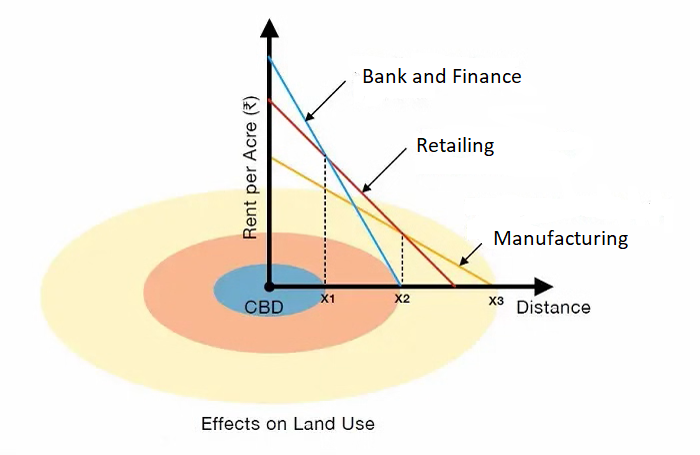
\includegraphics{images/bidrent.gpg.jpg}

The illustration shows three categories: The most expensive rent closest
to the centre is the Bank and finance district, followed by the retail
agglomeration areas and industrial sites furthest away from the central
point. Dental practices are service orientated thus depending on
population density and central activities. Opening hours are relay
outside of office hours. Production cost does not appear to be important
in this case since dentist is a public service. Hence, not dependent of
regular transportation of sales goods. The rent realized by the
landowner is the envelope of the three rent supply curves Capello
(2015).

From a Marshallian way of thinking dentists should cluster somewhere in
this pink area to reap maximum sales volume. Furthermore, they may also
increase their profits further out in to other retail agglomeration
area. The attractiveness might be high in these places due to economies
of scope. As the positive benefits from the Marshallian agglomeration
attributes play out. Subsequently, increasing profit by trading higher
transportation cost for lower rent. In addition fewer dentists to
compete with supporting the hotellings game theory whereas companies
more to achieve spatial monopoly McCann (2013).

\textbf{Gravitational models}

The centre attracts firms, people and activities. Furthermore, it
influence the central points in diverse ways such as commuter movements,
diffusion of knowledge, corporations and network and personal
relationship Capello (2015). More-so, they are generated by the
intensity of the flows generated between places Capello (2015). The
gravitational pull to a place of interest for a dentist will determine
how much sales can be generated by locating there. Several locations can
then be measures against each other to determine profit maximisation.

These models has the potential to measures the future attractiveness of
a place. Changes in infrastructure such as easier access to a place
might change the attractiveness of a place or move the flow of people.
Subserviently, increasing the gravitationally pull between the two
places. Furthermore, The model uses population and distance to measure
the attractiveness and relations between two places Capello (2015).
Furthermore, these models have predictive capacity and can be used to
estimate the potential impact. In particular, location of new productive
activity in an area Capello (2015). For instance predict where to build
a shopping centre Capello (2015). By taking these factors in to account
dentist could predict the most profitable locations in years to come by
predicting the amount of people that will move from one city to another
or tow different points of interest within a city.

\textbf{Retail Agglomeration and Economies of Shopping Centres}

Town and cities have long had shopping districts in which stores are
concentrated. To some extent such centre points were the result of
uncoordinated store-location decisions Brueckner (2011). Nevertheless,
not coincidentally according to Hotelling's theory (1929). He describes
the concentration of retail stores by a market desire to create a Nash
equilibrium. At this point all retailers expected sales maximisation
outcome cannot be improved by changing position. Contradictory to the
assumption that consumers will shop at the nearest retailer, they are
willing to travel significantly further to reach certain central places.
Marshall (1920) points out another explanation for this in his seminal
work on agglomeration. That being,intra-industry knowledge spillovers as
mechanisms leading to formation of industry cluster Nielsen et al.
(2021). In this case the dental industry information spillovers are
bounded in geographical space. Hence, the need to locate in close
proximity. That being the latest equipment, in order to work faster or
the right personnel to attract more patients. Another way to drive sales
in this area could be by dentist specialisation and patients referrals
between dentists.

Another important externalities expressed in Marshall (1920) theory is
market transactions. Whereas, geographical proximity reduces transaction
cost through several mechanism Nielsen et al. (2021). The market
transactions can be extended to the endogenous location of specialized
human capital Nielsen et al. (2021). ``It is well known among economists
and other social scientists that large cities have disproportionately
large shares of highly educated workers, and the trend has been growing
in recent decades.'' (\textbf{bakerBaker?}). Presumably, larger cities
would then be more attractive to dentists in terms of cost and quality
of specialised labour in smaller towns. Especially, those trying to
achieve spatial monopoly end up loosing profit by overpaying for labour
or in worst case scenario not finding enough dentists labour and end up
compromising on quality. In both cases growth potential would be
compromised.

Marshall also points out the competition within the geographical
location. Hence, the marketplace and business districts give consumers
low search and switching costs Capello (2015). The fact that owners of
stores seem to prefer highly concentrated shopping. More-so, it suggests
that the sales volumes outweigh the loss attributed to greater price
competition Capello (2015).

\textbf{Shopping Malls}

Owners of shopping malls ``orchestrate'' the process of retail
agglomeration that happens naturally in towns and cities Brueckner
(2011). Naturally, the same retail agglomeration and Nash equilibrium
may occur in shopping malls if not more intensely as the shops are in
closer proximity. Furthermore, the potential for more knowledge
spillovers, higher volume of market transaction and more competition.
When retail agglomeration is orchestrated by the owner of a shopping
mall, the strength and direction of such externalities are taken into
account Brueckner (2011). Much so, because the price of rent is
dependent on the overall revenue of a shopping mall. Hence, the owner of
the mall wants to choose the mix of stores and their sizes taking these
externalities, attributes and anchor stores attractiveness into account
Brueckner (2011).

The Norwegian retail market for alcoholic beverages is controlled by the
state monopoly. Anchor-stores such as the Wine-monopoly bring in a
higher volume of consumers (\textbf{lai2013Lai?}). For example, shoppers
visiting the Wine-monopoly in a mall may also visit a clothing store,
and even find it beneficial to use public services at the same time.
Nevertheless, they are limited in numbers and needs government approval.
Each municipality must apply to get the wine monopoly in their area. One
of the factors considered in this process is the death of city centre. A
possible reason for this is so called ``predatory malls'' which are
purposely built to overtake the exciting local market. Perhaps more so
if malls cater for cinema, restaurants, bars and other attributes in
conjunction with the city centre. Not to mention the upper hand of easy
road access and free parking.

\hypertarget{data}{%
\subsection{Data}\label{data}}

For this assignment we where provided with different geospatial data in
the geographic information software QGIS to calculate the relationship
of the different variables that might determine firm activity. This
geospatial data included Norwegian commune data which contained the
administrative boundaries of the Communes, presented in the software as
different divisions of lines that distinguish the different commune
boundaries. We where also provided with different point layers, such as
the geometric centers of communes, urban city centers or Central
Business Districts (CBD), all businesses in Norway which are regarded as
dental services, and all Norwegian shopping malls. We where also
provided with a QGIS layer with population density estimates, visualized
with 100x100 raster graphics.

To carry out a more complete data analysis of the influencing factors of
the activity of Norwegian dentist services, we had to collect more data
than what we already had been presented with. We firstly utilized QGIS
to calculate different other statistics and variables. Regarding the
Norwegian shopping malls layer we added the variable ``Wine-monopoly''
as a false/ true variable to determine which Norwegian malls had a hard
liquor store. We added the number of stores which are in each mall, to
use as an estimate for the malls sizes. The malls opening hours have
also been included in this layer. From SSB, we gathered data on the
average municipal sales per inhabitant in retailing for each Norwegian
commune. Lastly we created 2 kilometer buffer zones around dentists and
CBDs to determine population density in these areas.

After calculations in QGIS we transferred our data to RSTUDIO to do the
primary statistical analysis of our data. The data is then merged into
two different data frames. The first one containing Norwegian communes
as the unit of observation, which includes geometric commune centers to
the nearest mall, the retail per capita per commune, the different
commune numbers and the size of the nearest mall, including the true/
false ``Winemonopoly'' variable. The second data frame use dentists as
the unit of observations. This data frame include data on the distances
from CBD to dentists, distances from dentists to the nearest mall,
including variables of the mall size and the ``Winemonopoly'' variable,
different significant accounting figures for the different dentist
businesses, such as total sales revenue and EBIT (Earnings Before
Interests and Taxes). A summary of all the different variables can be
found in \textbf{?@tbl-1}, \textbf{?@tbl-2}, \textbf{?@tbl-3} and
\textbf{?@tbl-4}.

To obtain a first impression and a simple understanding of our data, we
have decided to make use of scatterplots. The scatterplot presented in
Figure~\ref{fig-1} show the relationship of average spending on retail
amongst inhabitants and the distance from geometrical commune centers to
nearest malls, which indicate that most malls are in a 50 km radius of
commune centers, and that Norwegians on average spend between 50
thousand to 120 thousand on retail.

We furthermore have used plots to look at the relationship between the
income of dentist's businesses and the distance from CBDs. The
scatterplot in Figure~\ref{fig-2} have some extreme figures of 1
billion+ income which we choose to ignore and deem as outliers, as we
notice that these observations are accounting figures for an entire
group of companies under the same legal name, and not individual
companies. By ignoring these outliers we are then left with the
scatterplot in Figure~\ref{fig-3}. This plot shows a tendency of a
negative relationship between the variables, which might suggest that
dentists might earn more closer to CBDs. The last scatterplots we have
chosen to calculate is concerning the relationship of dentists EBIT
which is earnings before interest and taxes, compared to their distances
to the nearest shopping mall in Figure~\ref{fig-4}. Just as the previous
scatterplot, we also see here a tendency of a negative relationship
between the variables. A decent number of dentists run at a loss, having
negative earnings before interest and taxes.

\hypertarget{econometric-approach}{%
\subsection{\texorpdfstring{\textbf{Econometric
Approach}}{Econometric Approach}}\label{econometric-approach}}

The questions addressed are related to the geographical space of Norway.
Norway is a country with relatively small population and large
heterogeneous land area. Furthermore, the population is decentralized
with the majority of population living in urban areas. This unique
spatial distribution of land might give a possible explanation to
diversions from the simple theoretical models used in this paper.
Whereas one of the assumptions are homogeneous landscape. Nevertheless,
the way economies are organised comes partly from the emergence of
centralities within a city. Transportation networks have the potential
to increase sprawl depending on how the urban system evolves gradually.

The results from the bid rent configuration from the city centre gave
the opportunity to explore other locations in each municipality's.
Having an urban system of multiple centres and applying the same logic
of the model to other retail agglomeration areas. Resulting in finding
relationships based on three different types of distance measurements.
Firstly, the distance between Dental Practice and CBD then, dentist and
other retail agglomeration areas and lastly amongst dentists. Finding
that most dentist are either located close to a City, Central Business
District or a shopping mall. Additionally, dentist also located close to
each other making some sort of industrial cluster. Supporting,
Marshall's agglomeration theory on knowledge spillovers, increasing the
sills to attract more patients.

Furthermore, when using the dentist income (y) and comparing the
distance from the mall (x), signs of patterns emerge showing that income
is greater when the dentist is placed closer to the shopping mall.
Furthermore, decreasing as the distance gets bigger. Faster
transportation can increase convenience of commuting, increasing rent
commuters from the city centre are willing to pay, and therefore
increasing the area of developed land without this being necessary
corresponding to an increase in population. Hence supporting findings;
when the distance reach around 10km from the mall the income starts to
increase before it decrease again around 20km. Also in line with the
Keynesian theory suggesting that this pattern might take place as the
transportation cost for individuals further away from the Shopping mall
does not increase to much by travelling the extra distance. Hotelling
also describes this case where the consumer are willing to travel
further to reach a certain central place.

According to the Alons's model dentist should locate in the retail area
for higher volume of sales. Dentist being placed further out in to other
retail agglomeration areas can also be a good strategy. However, the
dentist would then rely on the area having less competition so the rate
between competition and population density are proportional. Our
findings in QGIS shows that in areas of high population density, the
number of dentist also increase. The consumer/patient then has more to
choose between and the dentist also has a bigger scale of potential
customers. Where in smaller areas it is less competition and the dentist
would appear to have somewhat of a monopoly since the transportation
cost to the second closes dentist are noticeable higher.

Furthermore, being aware of the fact that going to the dentist is a
public services and most people get assigned to their closest dentist
based on their living address. This also takes away some of the
competition and would support placement in more rural areas. More-so, is
important to notice that when passed 18 years of age, you could risk
loosing your local public dentist due to lack of capacity. Suggesting
some dentist might seek closer to CBD areas to capture most of the
remaining part of the population. Business, public places and industry
can have a positive effect on revenue since this is areas where most of
the population spends their time during their day, either going to work,
school and other errand. Reducing the transportation cost for the
customer as they are already located in these areas even if they do not
live here.

The bid rent models are under the assumption that Dentists use spatial
completion to maximise profit. Nevertheless, the cost of dental care in
Norway can vary depending on a number of other factors such as the type
of treatment, the location of the dental practice and the dentist
experience and qualifications. The Norwegian Dental Association rate the
average cost of check ups is between four to eight hundred Norwegian
Krone's (\textbf{tannlege?}). Bertrand model also take price as
competitive advantage in to consideration.

Viser data noe om indikasjon på dyrere priser i nærheten av større byer
of hvor det er stedsbestemt monopol? Tjener tannleger i større byer mer?
Her kan vi også skrive om gravitasjons modeller.

Another Mashiallian point to be made could be the advantage of industry
clusters. Taken for granted that the data on Dentist includes both
``normal Dentists'' and specialist. Where in this case a ``normal
dentist'' would for example recommend one of their customers to go see a
specialist to get braces. The customer would then probably prefer to go
to the closes specialist. The access to work force in these areas would
also be good and will be within the same geographic area.

Shopping malls have a relatively short history in Norway, with the first
shopping mall opening in the late sixties. Prior to the most retail
activities took place in the city centre. Furthermore, these malls
typically featured a mix of shops, restaurants and entertainment
options, and they were often located in suburban areas or on the
outskirts of cities (\textbf{home-n?}). In resent years, there has been
a trend towards larger and more comprehensive shopping malls in Norway
(\textbf{home-n?}).

However, the growth of shopping malls in Norway has not been without
controversy. Some critics argue that the development of large shopping
malls has led to the decline of traditional shopping streets and local
businesses, while other raise concerns about the environmental impact of
these large scale commercial developments (\textbf{kanvin2014?}).

Information about Wine monopoly locations has also been studied in this
paper. As the wine monopoly are anchor stores they may affect the
attractiveness of the shopping mall (\textbf{kanvin2014?}). The
Norwegian government regulates the placements of wine monopoly stores in
shopping malls to prevent completion with town centres
(\textbf{omsorgsdepartementet2022?}). More importantly, the government
may take in to account the potential impact of exciting retail centres
in the region. This regional economic approach aim to promote
sustainable development and balance economic growth across the country
(\textbf{kanvin2014?}).

Hva viser informasjonen om vinmonopolet?

 
  \providecommand{\huxb}[2]{\arrayrulecolor[RGB]{#1}\global\arrayrulewidth=#2pt}
  \providecommand{\huxvb}[2]{\color[RGB]{#1}\vrule width #2pt}
  \providecommand{\huxtpad}[1]{\rule{0pt}{#1}}
  \providecommand{\huxbpad}[1]{\rule[-#1]{0pt}{#1}}

\begin{table}[ht]
\begin{centerbox}
\begin{threeparttable}
 
\setlength{\tabcolsep}{0pt}
\begin{tabular}{l l}


\hhline{>{\huxb{0, 0, 0}{0.8}}->{\huxb{0, 0, 0}{0.8}}-}
\arrayrulecolor{black}

\multicolumn{1}{!{\huxvb{0, 0, 0}{0}}c!{\huxvb{0, 0, 0}{0}}}{\huxtpad{6pt + 1em}\centering \hspace{6pt}  \hspace{6pt}\huxbpad{6pt}} &
\multicolumn{1}{c!{\huxvb{0, 0, 0}{0}}}{\huxtpad{6pt + 1em}\centering \hspace{6pt} Dentist Revenue \hspace{6pt}\huxbpad{6pt}} \tabularnewline[-0.5pt]


\hhline{>{\huxb{255, 255, 255}{0.4}}->{\huxb{0, 0, 0}{0.4}}-}
\arrayrulecolor{black}

\multicolumn{1}{!{\huxvb{0, 0, 0}{0}}l!{\huxvb{0, 0, 0}{0}}}{\huxtpad{6pt + 1em}\raggedright \hspace{6pt} (Intercept) \hspace{6pt}\huxbpad{6pt}} &
\multicolumn{1}{r!{\huxvb{0, 0, 0}{0}}}{\huxtpad{6pt + 1em}\raggedleft \hspace{6pt} 3616068.187 *** \hspace{6pt}\huxbpad{6pt}} \tabularnewline[-0.5pt]


\hhline{}
\arrayrulecolor{black}

\multicolumn{1}{!{\huxvb{0, 0, 0}{0}}l!{\huxvb{0, 0, 0}{0}}}{\huxtpad{6pt + 1em}\raggedright \hspace{6pt}  \hspace{6pt}\huxbpad{6pt}} &
\multicolumn{1}{r!{\huxvb{0, 0, 0}{0}}}{\huxtpad{6pt + 1em}\raggedleft \hspace{6pt} (373568.663)\hphantom{0}\hphantom{0}\hphantom{0} \hspace{6pt}\huxbpad{6pt}} \tabularnewline[-0.5pt]


\hhline{}
\arrayrulecolor{black}

\multicolumn{1}{!{\huxvb{0, 0, 0}{0}}l!{\huxvb{0, 0, 0}{0}}}{\huxtpad{6pt + 1em}\raggedright \hspace{6pt} DistComp \hspace{6pt}\huxbpad{6pt}} &
\multicolumn{1}{r!{\huxvb{0, 0, 0}{0}}}{\huxtpad{6pt + 1em}\raggedleft \hspace{6pt} -105.228\hphantom{0}\hphantom{0}\hphantom{0}\hphantom{0} \hspace{6pt}\huxbpad{6pt}} \tabularnewline[-0.5pt]


\hhline{}
\arrayrulecolor{black}

\multicolumn{1}{!{\huxvb{0, 0, 0}{0}}l!{\huxvb{0, 0, 0}{0}}}{\huxtpad{6pt + 1em}\raggedright \hspace{6pt}  \hspace{6pt}\huxbpad{6pt}} &
\multicolumn{1}{r!{\huxvb{0, 0, 0}{0}}}{\huxtpad{6pt + 1em}\raggedleft \hspace{6pt} (152.737)\hphantom{0}\hphantom{0}\hphantom{0} \hspace{6pt}\huxbpad{6pt}} \tabularnewline[-0.5pt]


\hhline{}
\arrayrulecolor{black}

\multicolumn{1}{!{\huxvb{0, 0, 0}{0}}l!{\huxvb{0, 0, 0}{0}}}{\huxtpad{6pt + 1em}\raggedright \hspace{6pt} DistMal \hspace{6pt}\huxbpad{6pt}} &
\multicolumn{1}{r!{\huxvb{0, 0, 0}{0}}}{\huxtpad{6pt + 1em}\raggedleft \hspace{6pt} -13619.260\hphantom{0}\hphantom{0}\hphantom{0}\hphantom{0} \hspace{6pt}\huxbpad{6pt}} \tabularnewline[-0.5pt]


\hhline{}
\arrayrulecolor{black}

\multicolumn{1}{!{\huxvb{0, 0, 0}{0}}l!{\huxvb{0, 0, 0}{0}}}{\huxtpad{6pt + 1em}\raggedright \hspace{6pt}  \hspace{6pt}\huxbpad{6pt}} &
\multicolumn{1}{r!{\huxvb{0, 0, 0}{0}}}{\huxtpad{6pt + 1em}\raggedleft \hspace{6pt} (32749.952)\hphantom{0}\hphantom{0}\hphantom{0} \hspace{6pt}\huxbpad{6pt}} \tabularnewline[-0.5pt]


\hhline{}
\arrayrulecolor{black}

\multicolumn{1}{!{\huxvb{0, 0, 0}{0}}l!{\huxvb{0, 0, 0}{0}}}{\huxtpad{6pt + 1em}\raggedright \hspace{6pt} SizeMall \hspace{6pt}\huxbpad{6pt}} &
\multicolumn{1}{r!{\huxvb{0, 0, 0}{0}}}{\huxtpad{6pt + 1em}\raggedleft \hspace{6pt} 10063.209 *\hphantom{0}\hphantom{0} \hspace{6pt}\huxbpad{6pt}} \tabularnewline[-0.5pt]


\hhline{}
\arrayrulecolor{black}

\multicolumn{1}{!{\huxvb{0, 0, 0}{0}}l!{\huxvb{0, 0, 0}{0}}}{\huxtpad{6pt + 1em}\raggedright \hspace{6pt}  \hspace{6pt}\huxbpad{6pt}} &
\multicolumn{1}{r!{\huxvb{0, 0, 0}{0}}}{\huxtpad{6pt + 1em}\raggedleft \hspace{6pt} (4523.296)\hphantom{0}\hphantom{0}\hphantom{0} \hspace{6pt}\huxbpad{6pt}} \tabularnewline[-0.5pt]


\hhline{}
\arrayrulecolor{black}

\multicolumn{1}{!{\huxvb{0, 0, 0}{0}}l!{\huxvb{0, 0, 0}{0}}}{\huxtpad{6pt + 1em}\raggedright \hspace{6pt} DistCBD \hspace{6pt}\huxbpad{6pt}} &
\multicolumn{1}{r!{\huxvb{0, 0, 0}{0}}}{\huxtpad{6pt + 1em}\raggedleft \hspace{6pt} 7969.413\hphantom{0}\hphantom{0}\hphantom{0}\hphantom{0} \hspace{6pt}\huxbpad{6pt}} \tabularnewline[-0.5pt]


\hhline{}
\arrayrulecolor{black}

\multicolumn{1}{!{\huxvb{0, 0, 0}{0}}l!{\huxvb{0, 0, 0}{0}}}{\huxtpad{6pt + 1em}\raggedright \hspace{6pt}  \hspace{6pt}\huxbpad{6pt}} &
\multicolumn{1}{r!{\huxvb{0, 0, 0}{0}}}{\huxtpad{6pt + 1em}\raggedleft \hspace{6pt} (9756.588)\hphantom{0}\hphantom{0}\hphantom{0} \hspace{6pt}\huxbpad{6pt}} \tabularnewline[-0.5pt]


\hhline{}
\arrayrulecolor{black}

\multicolumn{1}{!{\huxvb{0, 0, 0}{0}}l!{\huxvb{0, 0, 0}{0}}}{\huxtpad{6pt + 1em}\raggedright \hspace{6pt} X\_sum \hspace{6pt}\huxbpad{6pt}} &
\multicolumn{1}{r!{\huxvb{0, 0, 0}{0}}}{\huxtpad{6pt + 1em}\raggedleft \hspace{6pt} 13.257\hphantom{0}\hphantom{0}\hphantom{0}\hphantom{0} \hspace{6pt}\huxbpad{6pt}} \tabularnewline[-0.5pt]


\hhline{}
\arrayrulecolor{black}

\multicolumn{1}{!{\huxvb{0, 0, 0}{0}}l!{\huxvb{0, 0, 0}{0}}}{\huxtpad{6pt + 1em}\raggedright \hspace{6pt}  \hspace{6pt}\huxbpad{6pt}} &
\multicolumn{1}{r!{\huxvb{0, 0, 0}{0}}}{\huxtpad{6pt + 1em}\raggedleft \hspace{6pt} (7.925)\hphantom{0}\hphantom{0}\hphantom{0} \hspace{6pt}\huxbpad{6pt}} \tabularnewline[-0.5pt]


\hhline{}
\arrayrulecolor{black}

\multicolumn{1}{!{\huxvb{0, 0, 0}{0}}l!{\huxvb{0, 0, 0}{0}}}{\huxtpad{6pt + 1em}\raggedright \hspace{6pt} DistMal:SizeMall \hspace{6pt}\huxbpad{6pt}} &
\multicolumn{1}{r!{\huxvb{0, 0, 0}{0}}}{\huxtpad{6pt + 1em}\raggedleft \hspace{6pt} -106.204\hphantom{0}\hphantom{0}\hphantom{0}\hphantom{0} \hspace{6pt}\huxbpad{6pt}} \tabularnewline[-0.5pt]


\hhline{}
\arrayrulecolor{black}

\multicolumn{1}{!{\huxvb{0, 0, 0}{0}}l!{\huxvb{0, 0, 0}{0}}}{\huxtpad{6pt + 1em}\raggedright \hspace{6pt}  \hspace{6pt}\huxbpad{6pt}} &
\multicolumn{1}{r!{\huxvb{0, 0, 0}{0}}}{\huxtpad{6pt + 1em}\raggedleft \hspace{6pt} (724.299)\hphantom{0}\hphantom{0}\hphantom{0} \hspace{6pt}\huxbpad{6pt}} \tabularnewline[-0.5pt]


\hhline{}
\arrayrulecolor{black}

\multicolumn{1}{!{\huxvb{0, 0, 0}{0}}l!{\huxvb{0, 0, 0}{0}}}{\huxtpad{6pt + 1em}\raggedright \hspace{6pt} DistCBD:X\_sum \hspace{6pt}\huxbpad{6pt}} &
\multicolumn{1}{r!{\huxvb{0, 0, 0}{0}}}{\huxtpad{6pt + 1em}\raggedleft \hspace{6pt} -1.105\hphantom{0}\hphantom{0}\hphantom{0}\hphantom{0} \hspace{6pt}\huxbpad{6pt}} \tabularnewline[-0.5pt]


\hhline{}
\arrayrulecolor{black}

\multicolumn{1}{!{\huxvb{0, 0, 0}{0}}l!{\huxvb{0, 0, 0}{0}}}{\huxtpad{6pt + 1em}\raggedright \hspace{6pt}  \hspace{6pt}\huxbpad{6pt}} &
\multicolumn{1}{r!{\huxvb{0, 0, 0}{0}}}{\huxtpad{6pt + 1em}\raggedleft \hspace{6pt} (1.065)\hphantom{0}\hphantom{0}\hphantom{0} \hspace{6pt}\huxbpad{6pt}} \tabularnewline[-0.5pt]


\hhline{>{\huxb{255, 255, 255}{0.4}}->{\huxb{0, 0, 0}{0.4}}-}
\arrayrulecolor{black}

\multicolumn{1}{!{\huxvb{0, 0, 0}{0}}l!{\huxvb{0, 0, 0}{0}}}{\huxtpad{6pt + 1em}\raggedright \hspace{6pt} N \hspace{6pt}\huxbpad{6pt}} &
\multicolumn{1}{r!{\huxvb{0, 0, 0}{0}}}{\huxtpad{6pt + 1em}\raggedleft \hspace{6pt} 1364\hphantom{0}\hphantom{0}\hphantom{0}\hphantom{0}\hphantom{0}\hphantom{0}\hphantom{0}\hphantom{0} \hspace{6pt}\huxbpad{6pt}} \tabularnewline[-0.5pt]


\hhline{}
\arrayrulecolor{black}

\multicolumn{1}{!{\huxvb{0, 0, 0}{0}}l!{\huxvb{0, 0, 0}{0}}}{\huxtpad{6pt + 1em}\raggedright \hspace{6pt} R2 \hspace{6pt}\huxbpad{6pt}} &
\multicolumn{1}{r!{\huxvb{0, 0, 0}{0}}}{\huxtpad{6pt + 1em}\raggedleft \hspace{6pt} 0.008\hphantom{0}\hphantom{0}\hphantom{0}\hphantom{0} \hspace{6pt}\huxbpad{6pt}} \tabularnewline[-0.5pt]


\hhline{>{\huxb{0, 0, 0}{0.8}}->{\huxb{0, 0, 0}{0.8}}-}
\arrayrulecolor{black}

\multicolumn{2}{!{\huxvb{0, 0, 0}{0}}l!{\huxvb{0, 0, 0}{0}}}{\huxtpad{6pt + 1em}\raggedright \hspace{6pt} Note:  *** p $<$ 0.001;  ** p $<$ 0.01;  * p $<$ 0.05 T statistics in brackets. \hspace{6pt}\huxbpad{6pt}} \tabularnewline[-0.5pt]


\hhline{}
\arrayrulecolor{black}
\end{tabular}
\end{threeparttable}\par\end{centerbox}

\end{table}
 

\hypertarget{conclusion}{%
\subsection{Conclusion}\label{conclusion}}

\hypertarget{references}{%
\subsection{References}\label{references}}

\hypertarget{appendix}{%
\subsection{Appendix}\label{appendix}}

\begin{tabular}{l|l|l|l|l|l|l}
\hline
  &     knr &    DistMal &    HubName & Turnover\_capita\_retail &    SizeMall &  Winemonopoly\\
\hline
 & Length:435 & Min.   : 0.01854 & Min.   :  6.0 & Min.   : 17366 & Min.   :  2.00 & Min.   :0.0000\\
\hline
 & Class :character & 1st Qu.: 9.41403 & 1st Qu.:220.0 & 1st Qu.: 59250 & 1st Qu.: 13.00 & 1st Qu.:0.0000\\
\hline
 & Mode  :character & Median :18.87373 & Median :291.0 & Median : 83203 & Median : 25.00 & Median :1.0000\\
\hline
 & NA & Mean   :23.82982 & Mean   :280.8 & Mean   : 84719 & Mean   : 37.22 & Mean   :0.5701\\
\hline
 & NA & 3rd Qu.:32.67127 & 3rd Qu.:363.0 & 3rd Qu.:106257 & 3rd Qu.: 50.00 & 3rd Qu.:1.0000\\
\hline
 & NA & Max.   :98.37355 & Max.   :424.0 & Max.   :218728 & Max.   :206.00 & Max.   :1.0000\\
\hline
 & NA & NA & NA & NA & NA's   :124 & NA's   :107\\
\hline
\end{tabular}

\begin{tabular}{l|l|l|l|l}
\hline
  &   Antall.ans &   Driftsres &   Sum.salgsi &   latlong\\
\hline
 & Min.   :   0.00 & Min.   :-30319000 & Min.   :    -28000 & Length:5740\\
\hline
 & 1st Qu.:   1.00 & 1st Qu.:    -5000 & 1st Qu.:    658250 & Class :character\\
\hline
 & Median :   1.00 & Median :   330000 & Median :   3176500 & Mode  :character\\
\hline
 & Mean   :  39.26 & Mean   :  4842620 & Mean   :  50123495 & NA\\
\hline
 & 3rd Qu.:   3.00 & 3rd Qu.:  1201750 & 3rd Qu.:   6248250 & NA\\
\hline
 & Max.   :6870.00 & Max.   :108100000 & Max.   :1058102000 & NA\\
\hline
 & NA & NA's   :3838 & NA's   :3838 & NA\\
\hline
\end{tabular}

\begin{tabular}{l|l|l|l|l}
\hline
  &    DistCBD &    DistMal &     X\_sum &    DistComp\\
\hline
 & Min.   :  0.0046 & Min.   :  0.0008 & Min.   :    0 & Min.   :    0.0\\
\hline
 & 1st Qu.:  1.3912 & 1st Qu.:  0.3145 & 1st Qu.: 6129 & 1st Qu.:    0.0\\
\hline
 & Median :  6.7067 & Median :  0.9164 & Median :14602 & Median :    0.0\\
\hline
 & Mean   : 20.5000 & Mean   :  4.6331 & Mean   :22455 & Mean   :  614.4\\
\hline
 & 3rd Qu.: 19.8885 & 3rd Qu.:  2.5220 & 3rd Qu.:28904 & 3rd Qu.:  197.7\\
\hline
 & Max.   :470.1005 & Max.   :105.8867 & Max.   :92591 & Max.   :60577.8\\
\hline
\end{tabular}

\begin{tabular}{l|l|l}
\hline
  &    SizeMall &  Winemonopoly\\
\hline
 & Min.   :  1.0 & Min.   :0.0000\\
\hline
 & 1st Qu.: 21.0 & 1st Qu.:0.0000\\
\hline
 & Median : 40.0 & Median :1.0000\\
\hline
 & Mean   : 51.1 & Mean   :0.6429\\
\hline
 & 3rd Qu.: 70.0 & 3rd Qu.:1.0000\\
\hline
 & Max.   :206.0 & Max.   :1.0000\\
\hline
 & NA's   :1388 & NA's   :1274\\
\hline
\end{tabular}

\begin{verbatim}
Warning: Removed 124 rows containing missing values (geom_point).
\end{verbatim}

\begin{figure}

{\centering 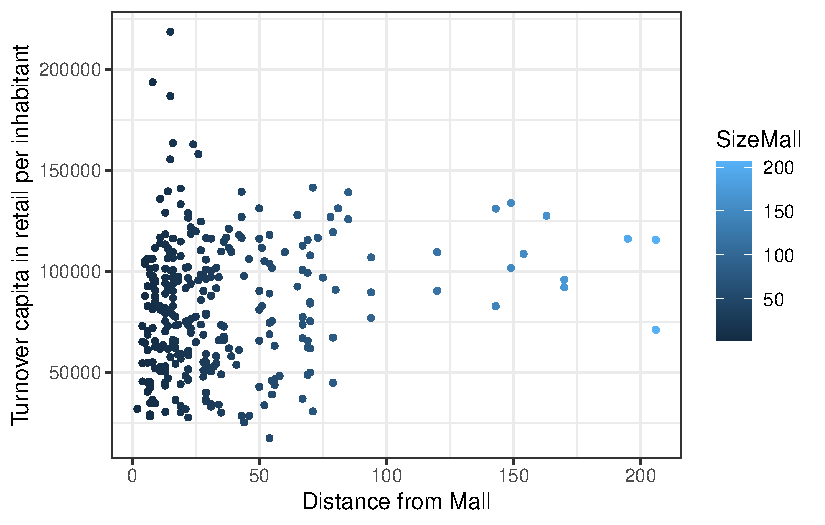
\includegraphics{Retail-Agglomeration_abstract_introduction_theori_econometric_approach_files/figure-pdf/fig-1-1.pdf}

}

\caption{\label{fig-1}Capita in retail compared to mall distance}

\end{figure}

\begin{verbatim}
Warning: Removed 3838 rows containing missing values (geom_point).
\end{verbatim}

\begin{figure}

{\centering 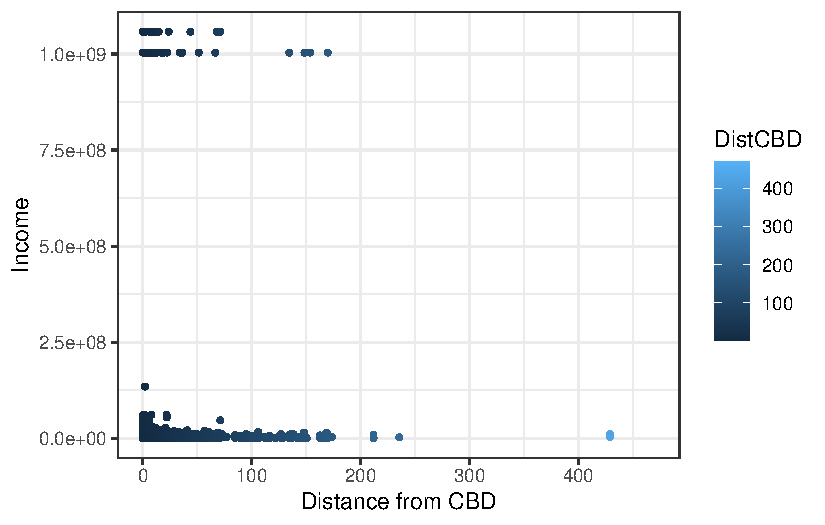
\includegraphics{Retail-Agglomeration_abstract_introduction_theori_econometric_approach_files/figure-pdf/fig-2-1.pdf}

}

\caption{\label{fig-2}Dentist income compared to CBD distance}

\end{figure}

\begin{figure}

{\centering 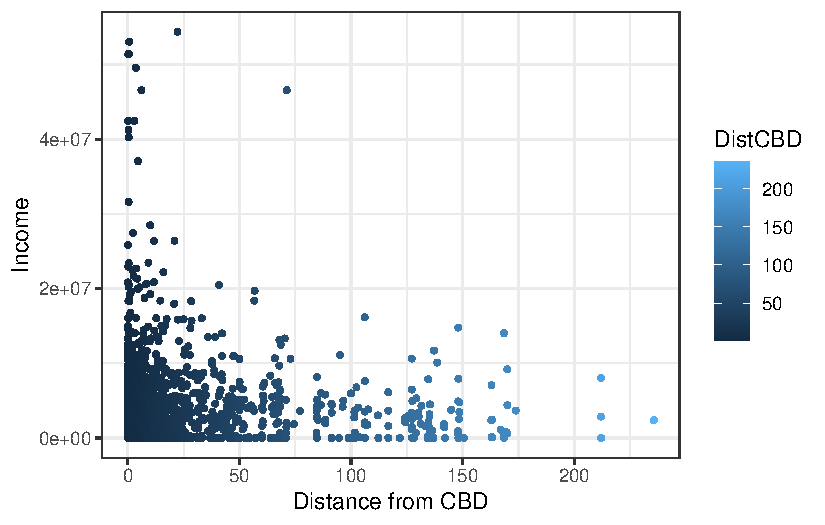
\includegraphics{Retail-Agglomeration_abstract_introduction_theori_econometric_approach_files/figure-pdf/fig-3-1.pdf}

}

\caption{\label{fig-3}Dentist income compared to CBD distance}

\end{figure}

\begin{verbatim}
Warning: Removed 3838 rows containing missing values (geom_point).
\end{verbatim}

\begin{figure}

{\centering 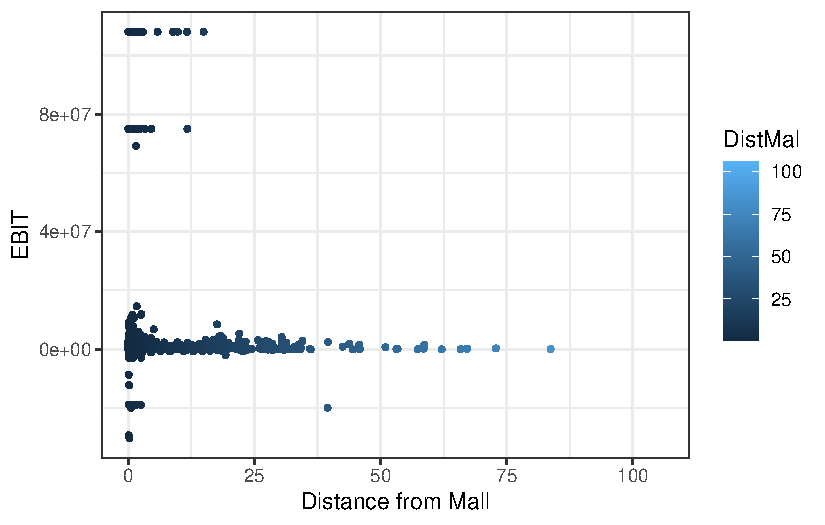
\includegraphics{Retail-Agglomeration_abstract_introduction_theori_econometric_approach_files/figure-pdf/fig-4-1.pdf}

}

\caption{\label{fig-4}Dentist EBIT compared to Mall distance}

\end{figure}

\hypertarget{refs}{}
\begin{CSLReferences}{1}{0}
\leavevmode\vadjust pre{\hypertarget{ref-brueckner2011}{}}%
Brueckner, Jan K. 2011. \emph{Lectures on Urban Economics}. MIT Press.

\leavevmode\vadjust pre{\hypertarget{ref-capello2011}{}}%
Capello, Roberta. 2011. {``{[}PDF{]}location, Regional Growth and Local
Development Theories,''} January.
\url{https://www.academia.edu/48547951/_PDF_Location_Regional_Growth_and_Local_Development_Theories}.

\leavevmode\vadjust pre{\hypertarget{ref-capello2015}{}}%
---------. 2015. \emph{Regional Economics}. 2nd ed. Routledge.
\url{https://doi.org/10.4324/9781315720074}.

\leavevmode\vadjust pre{\hypertarget{ref-davis2020}{}}%
Davis, Donald R., and Jonathan I. Dingel. 2020. {``The Comparative
Advantage of Cities.''} \emph{Journal of International Economics} 123
(March): 103291. \url{https://doi.org/10.1016/j.jinteco.2020.103291}.

\leavevmode\vadjust pre{\hypertarget{ref-duranton2004}{}}%
Duranton, Gilles, and Diego Puga. 2004. {``Chapter 48 -
Micro-Foundations of Urban Agglomeration Economies.''} In \emph{Handbook
of Regional and Urban Economics}, edited by J. Vernon Henderson and
Jacques-François Thisse, 4:2063--2117. Cities and Geography. Elsevier.
\url{https://doi.org/10.1016/S1574-0080(04)80005-1}.

\leavevmode\vadjust pre{\hypertarget{ref-mccann2013}{}}%
McCann, Philip. 2013. \emph{Modern Urban and Regional Economics}. Second
edition. Oxford University Press.

\leavevmode\vadjust pre{\hypertarget{ref-nielsen2021}{}}%
Nielsen, Bo Bernhard, Christian Geisler Asmussen, Cecilie Dohlmann
Weatherall, and Ditte Håkonsson Lyngemark. 2021. {``Marshall Vs Jacobs
Agglomeration and the Micro-Location of Foreign and Domestic Firms.''}
\emph{Cities} 117 (October): 103322.
\url{https://doi.org/10.1016/j.cities.2021.103322}.

\leavevmode\vadjust pre{\hypertarget{ref-puga2010}{}}%
Puga, Diego. 2010. {``THE MAGNITUDE AND CAUSES OF AGGLOMERATION
ECONOMIES.''} \emph{Journal of Regional Science} 50 (1): 203--19.
\url{https://doi.org/10.1111/j.1467-9787.2009.00657.x}.

\end{CSLReferences}



\end{document}
